\chapter{Installation}\label{sec:install}

\paragraph{}The FA$\mu$ST project is based on an C++ library available for both UNIX and Windows environments and is delivered with a Matlab wrapper. CMake has been choose to build the project FA$\mu$ST because it is an open-source, cross-platform family of tools designed to build, test and package software.

\paragraph{}First section \ref{sec:UnixInstall} explains how to install the project FA$\mu$ST for UNIX platform and second section \ref{sec:WinInstall} corresponds to the Windows installation. 

\section{Unix platform}\label{sec:UnixInstall}

\subsection{Getting Started}\label{sec:GettingStarted}

\subsubsection{Required tools}\label{sec:RequiredTools}

\begin{itemize}
\item CMake : (tested with version 3.4.3 cf. website \url{https://cmake.org/})
\item Matlab : (tested with version 2014 and 2015)
The use of the mex function in Matlab requires that you have a third-party compiler installed on your system. The latest version of Matlab (2016a in our case) only supports up to GCC 4.7 (see \url{http://fr.mathworks.com/support/compilers/R2016a/index.html?sec=glnxa64} for more detail). Please adjust your version of GCC compiler in order to run the installation properly. 
You must too have matlab in your environment PATH. If not please add. 

\item -OPTIONAL- The use of GPU process in FAUST project required the drivers for NVIDIA and CUDA install. You must have nvcc in your environment PATH. If not please add.
\end{itemize}

\paragraph{}Please export following variable:
\begin{itemize}
\item CC with gcc (example: "\texttt{export CC='/usr/lib64/ccache/gcc'}") 
\item CXX with g++ (example: "\texttt{export CXX=/usr/lib64/ccache/g++}
\end{itemize}

\subsubsection{Required packages}\label{sec:RequiredPackages}

\paragraph{}Here is a list of packages used with Faust project. Normally, the installation of this packages are automatically done (see the directory "./externals").
\begin{itemize}
\item eigen
\item openBlas
\item xml2
\item matio
\end{itemize}

\subsubsection{Basic build and installation}\label{sec:UnixBuildInstall}
\paragraph{}When prerequisities listed in precedent sections are checked, the FA$\mu$ST installation can be done : 

\begin{itemize}
\item Download the FA$\mu$ST package on the website :  \url{http://faust.gforge.inria.fr/}
\item Open a command terminal
\item Place you in the FA$\mu$ST directory, and type the following commands : 
\begin{lstlisting}
mkdir build
cd build
cmake ..
make
sudo make install
\end{lstlisting}
\end{itemize}

\paragraph{}When using the \texttt{cmake} command to generate the build system, Cmake performs a list of tests to determine the system configuration and manage the build system. If the configuration is correct then the build system is generated and written. In this case the three last lines of the console log of cmake command should be: \\
\texttt{... \\
-- Configuring done \\
-- Generating done \\
-- Build files have been written to: ./build}

\paragraph{}The command \texttt{make} will compile the build files.

\paragraph{}The command \texttt{make install} will install in default directory.



\subsection{Custom - Advanced Installation}\label{sec:UnixCustomInstall}

\paragraph{}The project FA$\mu$ST can be configured with optional parameters, for example if you want to install FA$\mu$ST in a different folder or to enable the parallel computing using multithread capacities provided by the OS. This build system can be parametrized using the Cmake Graphical User Interface, or the Cmake command line tools. 

\paragraph{}The Cmake Graphical User Interface ccmake allows you to selected option input. When using the \texttt{ccmake} command in your build directory, the Cmake GUI appears in the console (see figure \ref{fig:ccmake}).

\begin{figure}[!htbp]
\label{fig:ccmake}
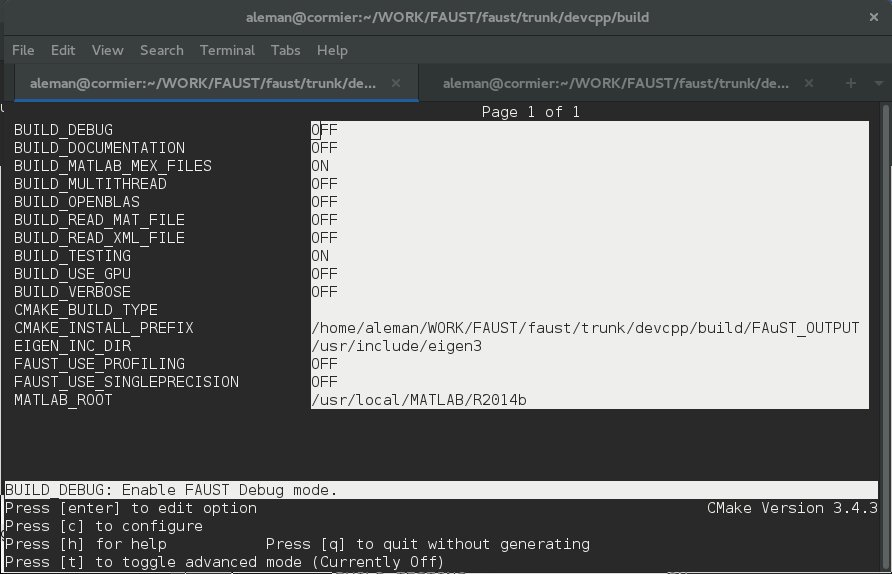
\includegraphics[scale=0.5]{images/ccmake.jpg}
\end{figure}

\paragraph{}When scrolling on a value and pressing [enter], this value can be edited, the black underlaid row displays some information about the option and required path to create the build system. In the case of an option press [enter] to toggle the ON/OFF values.
\paragraph{}After choosing options for the build and setting the required fields, press [c] to configure. The configuration of the build system is checked again by Cmake, at the end of this check if the build settings are correct, you can press [g] in order to generate the build system.
	

\paragraph{} The command line cmake can take some option input. Here is the list of available options: 
\texttt{$cmake\ ..\ -D<BUILD\_NAME>=<ON/OFF>$}

\begin{itemize}
\item BUILD\_TESTING : Enable the ctest option (default value is ON)
\item BUILD\_DOCUMENTATION : Generating the doxygen documentation (default value is OFF)  
\item BUILD\_MULTITHREAD : Enable multithread with OpenMP Multithreading (default value is OFF)
\item BUILD\_VERBOSE : Enable verbose option when compile (-v) (default value is OFF)
\item BUILD\_DEBUG : Enable FAUST Debug mode (default value is OFF )
\item BUILD\_USE\_GPU : Using both CPU and GPU process ( default value is OFF)
\item BUILD\_MATLAB\_MEX\_FILES : Enable building Matlab MEX files (default value is ON)
\item BUILD\_OPENBLAS : Using openBLAS for matrix and vector computations (default value is OFF )
\item BUILD\_READ\_XML\_FILE : Using xml2 library to read xml files (default value is OFF)
\item BUILD\_READ\_MAT\_FILE : Using matio library to read mat files (default value is OFF)
\end{itemize}

\paragraph{}Following the selected option, the cmake installer automatically checks the dependent component (library OpenBlas, eigen, matio, libxml2).  






\section{Windows platform}\label{sec:WinInstall}

\subsection{Prerequisities for installation}\label{sec:WinPrerequisitiesInstall}
The installation of the FA$\mu$ST project depends on other components to be installed in order to run properly. 
\begin{enumerate}

\item \textbf{Install CMake} for building the FAUST project. 
In \url{https://cmake.org/download/}, download Binary distributions correspond to your environment (in our case  cmake-3.6.1-win64-x64.zip)
The directory of binary must be add to the environment PATH of your system if you want to use the cmake command line tool. 

\item \textbf{Install 7-Zip} \url{http://www.7-zip.org/} . 7-Zip is a file archiver used for external library

\item \textbf{Install Matlab} if not already done (MATLAB R2015b in our case).

Note for the case of the use of compiler MinGW : In Matlab, you must install MinGW version 4.9.2 from MATLAB using the \textbf{ADDON menu}. For more detail, please follow the instruction given in following link :  
\url{http://fr.mathworks.com/help/matlab/matlab_external/install-mingw-support-package.html}. For that, you must have a id session for Mathwork. It is easy to create. 
Current this latest step, an environment variable called MW\_MINGW64\_LOC is automatically generated. 


\item \textbf{Install C++ Compiler:} Both \textbf{Microsoft visual C++} and \textbf{MinGW "Minimalist GNU for Windows"} compiler have been tested. The version of this compilers must be coherent with the version of your Matlab version. Here is the compiler installation corresponding to Matlab 2014 and 2015. If you use an other version of Matlab, please refers to the Mathworks website \url{http://fr.mathworks.com/support/compilers/<R20XXa>}.

\paragraph{}For \textbf{Microsoft visual C++} installation :
\begin{itemize}
\item Download and install Microsoft Visual C++ 2013 professional
% \item Download and install Microsoft .NET Framework 4
% \item Download and install Microsoft SDK 7.1
\end{itemize}

\paragraph{}For \textbf{MinGW} installation :
\begin{itemize}
\item Download Mingw in \url{https://sourceforge.net/projects/mingw/files/latest/download?source=files}
\item Launch install file and choose MINGW version 4.9.2 for mexFunction compatibility 
\item The directory of binary must be add to the environment PATH. 

\item Note for make tool : In a terminal command, type "make". if it doesn't exist, please check if make.exe is present in MINGW install directory. if not, you can copy and rename mingw32-make.exe to make.exe
\end{itemize}



\item In your environment PATH, please verify and add following components :

\begin{itemize}
\item matlab.exe (example: "C:$\setminus$Program Files$\setminus$MATLAB$\setminus$R2015b$\setminus$bin")
\item 7z.exe (example: "C:$\setminus$prog$\setminus$7-Zip")
\item cmake.exe (example: "C:$\setminus$Users$\setminus$ci$\setminus$Documents$\setminus$library$\setminus$cmake-3.6.0-win64-x64$\setminus$bin")
\item In case of the use of MinGW compiler : gcc.exe (example: "C:$\setminus$mingw-w64$\setminus$mingw64$\setminus$bin")
\end{itemize}
\end{enumerate}


\subsection{FAUST installation}\label{sec:WinFaustInstall}
When prerequisities listed in precedent section \ref{sec:WinPrerequisitiesInstall} are checked, the FA$\mu$ST installation can be done. 
Download the FA$\mu$ST package on the website :  \url{http://faust.gforge.inria.fr/}


\paragraph{}In the case of MinGW compiler :
Open a command terminal and place you in the FAUST directory. Type the following commands : 
\begin{lstlisting}
mkdir build
cd build
cmake -G "MinGW Makefiles" .. 
make
make install
\end{lstlisting}

\paragraph{}In the case of Microsoft Visual Studio 2013 compiler using the command terminal :
Open a command terminal and place you in the FAUST directory. Type the following commands : 
\begin{lstlisting}
mkdir build
cd build
cmake -G "Visual Studio 12 2013" .. 
cmake --build . --config "Release" --target "install"
\end{lstlisting}


\paragraph{}In the case of Microsoft Visual Studio 2013 compiler using the Graphical Users Interfaces:
\begin{lstlisting}
open application cmake-GUI.exe located in cmakeTool/bin
select input source to ./FAUST_Root/
select output build in ./FAUST-ROOT/build
configure
generate

open Faust.visualstudio
generated ALL_BUILD
generate INSTALL
generate CTEST to verify all is ok
\end{lstlisting}



\subsection{Optional - Advanced Installer}\label{sec:WinOptionalInstall}

progress... 



